\documentclass[12pt, a4paper,titlepage]{article}

\usepackage{hyperref}
\usepackage{fancyhdr}
\usepackage{url}
\usepackage{graphicx}


\title{Development of a Component Based Share Trader Application}
\author{S. Dixon
        \\\href{mailto:40056761@live.napier.ac.uk}{40056761@live.napier.ac.uk}
        \\Edinburgh Napier University
        \\School Of Computing
        \\}

\date{April 2018}
\lhead{SET11504 - Advanced Software Development}
\rhead{40056761}


\begin{document}
\maketitle

\tableofcontents
\newpage


\section{Introduction}
The purpose of this report is to document and evaluate the processes and
techniques utilised in the construction of a component based Share Trader
desktop application.

The Share Trader system is a prototype application that aims to aggregate and
display information relating to shares, trades, shareholders, brokers, etc. in
a single, easy to use application. 

The caveat of this development project is that the Share Trader system had to
constructed using Component Based Software Engineering (CBSE) techniques.

This report documents how software components were identified, modified and
combined to construct the Share Trader system - an evaluation of the process'
and techniques is also provided.


\section{Tools and Technologies}
When undergoing the development of a software project, the tools utilised can
greatly alter the time and effort required to implement, test and deploy a
system.
This project utilised the technologies listed in Table \ref{table-tech} to
implement the Share Trader System.
Additionally, Table \ref{table-tool} lists the tools that aided in development
of the Share Trader system.

\begin{table}[h]
    \centering
    \begin{tabular}{|l|l|}
        \hline
        \textbf{Technology}  & \multicolumn{1}{c|}{\textbf{Purpose}} \\ \hline
        Java        & User interface and logic     \\ \hline
        MySQL       & Back end database            \\ \hline
        Gradle      & Build tool                   \\ \hline
        \LaTeX      & Documentation                \\ \hline
    \end{tabular}
    \caption{Share Trader Technologies}
    \label{table-tech}
\end{table}

\begin{table}[h]
    \centering
    \begin{tabular}{|l|l|}
        \hline
        \multicolumn{1}{|c|}{\textbf{Tool}} &
        \multicolumn{1}{c|}{\textbf{Purpose}} \\ \hline
        IntelliJ Idea                       & Java development and testing
        \\ \hline
        MySQL Workbench                     & Database configuration
        \\ \hline
        Git                                 & Version control management
        \\ \hline
    \end{tabular}
    \caption{System Development Tools}
    \label{table-tool}
\end{table}


\subsection{Java, IntelliJ Idea, and Gradle}
Java was elected as the primary development language for this project in
accordance with the project specification document.

JetBrains is an organisation that has produced a number of Integrated
Development Environments (IDE) for a range of different languages and
frameworks.
IntelliJ Idea is JetBrains' Java IDE, offering a number of in-built tools and
features to aid in the development, testing and debugging of Java
applications \cite{Idea}.
IntelliJ Idea was selected as the primary development platform primarily due to
the author's familiarity with the system.
One of IntelliJ Idea's features that was utilised heavily during the course
of this project was its in-built User Interface (UI) building tool, which
allowed for quick and simple construction and alteration of Java Swing forms
used throughout the system.

Grade is Java compatible build tool that aids in the automated compilation
and linking of source code and libraries into a single application
\cite{Gradle}.
Gradle was utilised in this project as the Share Trader system was developed
using multiple machines, with various differing operating systems and system
configurations.
Use of Gradle was able to reduce the complexity of configuring and compiling
source code using multiple systems by utilising its various automation tools and
plug-ins.

\subsection{MySQL and MySQL Workbench}
The Share Trader application required some manner of data persistence in order
to properly operate.
MySQL is an open-source Relation Database Management System (RDBMS) that was
selected to fulfil the role of providing data persistence \cite{Mysql}.
MySQL was chosen as it is cross platform and requires no finance commitment
to utilise.
A simple prototype database schema was created to allow the various features
of the Share Trader system to be implemented, tested, and demonstrated.
An ER diagram of project's schema is visible in Appendix \ref{ap-schema}.

MySQL Workbench is a database configuration tool that operates in a similar
style as a traditional IDE \cite{Workbench}.
MySQL Workbench was used to configure the MySQL database instance and to
confirm that the SQL queries that were later incorporated into the Share
Trader system proper.


\section{Component Mining}
When undertaking a CBSE project, the process of identifying potentially usable
software components is often referred to as Component Mining.  
Component Mining consists of identifying potentially useful units of software
from existing sources - allowing a developer to access a range of features
that they can be combined into a finished system.

Components can be sourced from previous projects, open-source code
repositories, or stand-alone libraries. 
Having access to a wide range of components can allow a prototype system to be
quickly assembled and tested to prove a concept.

\subsection{Legacy System}
The source code to a legacy system was provided from which potential
components could be identified and possibly incorporated into the Share Trader
system.  
The legacy code was an implementation of E-Store system and consisted of a
number of Java Swing forms that were populated with information from a local
database.

While the business logic of the legacy system was not reusable, much of the
graphical user interface (GUI) had the potential to be reimplemented as part of
the new Share Trader system.

\subsubsection{Main Menu}
The legacy system’s GUI consisted of a main menu featuring a number of
buttons, each of which opened a new window to provide access to a different
E-Store feature; such as inventory management, delivery status, and customer
financial status.  
The intuitive nature of the menu system made it an ideal component to utilise
in the new Share trader system - which would also consist of a number features
that a user would have to navigate between.

\subsubsection{Display Forms}
When one of the legacy system’s menu buttons was clicked, a new GUI form would
open to display data and interactive elements to the user.  
While the business logic of these forms was incompatible with the Share
Trader system, the tables used to display data, the text fields used for user
input, and the buttons utilised to submit searches and close the forms could
be altered to work with the new system.

\subsubsection{Database Connector}
Apart from the GUI elements, the legacy system also featured an interface
which defined the method names and signatures required to connect, close, and
query a database instance. 
While the legacy system’s concrete implementations of the database connector
were not be reusable - the interface itself could be used to implement a 
database connection in the new Share Trader application.

\subsection{Previous Projects}
A previous data analysis project completed by the author utilised property
files to augment and control access to a database, without the need to alter
or recompile source code \cite{Dixon2017}.  
This component would allow the Share Trader system
to access different databases as required, or allow a developer to connect to
one database for testing and another for deployment.

\subsection{Open-source Libraries}
Software components are often published as stand-alone libraries, which can be
be linked and incorporated into a system. 
One such library that was considered in this project was the JDatePicker - a
GUI component that creates a interactive calendar, allowing a user to select a
date \cite{Jdate}. 
This component was considered as the project's specification brief stated that
users should be able to search and sort trading information based on certain
criteria - date included. 
By utilising a pre existing date picker, development and testing time could be
potentially saved.


\section{Component Selection}
From the previously mentioned components identified  during the
component mining process, the following were utilised in the final system:
\begin{itemize}
\item Database Connection Interface
\item Database Connection Manager
\item JDatePicker
\item GUI Display Forms
\end{itemize}

\subsection{Database Connection Interface}
The database connection interface not only provided sensible methods but also
allows a system to take advantage of the Object Orientated (OO) principal of
principal of polymorphism - allowing a differing implementation of the
interface to be substituted for one another. 
In the case of the Share Trader system, the database connection interface was
implemented as a MySQL connection but implementations for any kind of data
persistence system could be implemented and selected at run time by
utilising the existing database connection interface.

\subsection{Database Connection Manager}
The database connection manager was selected for use in the Share Trader
system primarily for developmental reasons.
The database management system allows users to utilise a configuration
(config) file to define the address, user, and password needed to connect to a
database instance. 
As the Share Trader system was being developed across multiple
devices each with differing database set-ups, the database management system
allowed development to continue by simply editing a config file, rather than
source-code.  
The database management system also had the benefit of
allowing a user to define a primary and secondary database to which the system
could connect. 
This feature can prove useful when testing a system, as the system can connect
to a database set up as a testing environment, rather than performing
potentially devastating operations upon the data required for final deployment
and operation.

\subsection{JDatePicker}
The JDatePicker is an open-source component that allows a user to select a
date using a simple, clickable pop-up calendar.
The JDatePicker has been developed using Java Swing components - meaning it is
compatible with the other GUI elements that were mined from the legacy system's
codebase.
The JDatePicker offers a number of customisation options to alter how the
picker operates.
One such alteration is the choice to return selected dates in a SQL query
compatible format - ideal for the proposed implementation of the Share Trader
system.  
Another benefit of the JDatePicker is that the author of the component has
thoroughly tested and verified that the widget is working correctly. 
These verifiable tests reduce the time required to test the Share Trader system
as there is no need to retest a component that has already been verified as
working.

\subsection{GUI Display Forms}
The legacy system provided a substantial amount of inspiration of how the new
Share Trader system should be implemented. 
The simple and intuitive design of the legacy system’s main menu provided a
foundation for the Share Trader system - assuming a few minor amendments were
made to the labelled buttons.
Similar adjustments could be made to the forms used to display information
tables.  
By reusing existing components from the legacy system, a substantial
amount of development time could theoretically be saved - utilising the work
of others can greatly mitigate development pressure by reducing the amount of
responsibility on a single person or team.


\section{Component Adaptation}
In order to comply with the project specification, the  Share Trader system
had to be constructed with reusable components that were JavaBean compliant.
This meant that the potential components identified during Component Mining
and Selection
processes  required a degree of amendment to match the JavaBean standard. 

\subsection{JavaBeans}
A JavaBean is a class that complies to a standardised convention, meaning that
a business system that is aware of said class’s parameters can automate the
instantiation of the class and it’s parameters. 
A JavaBean can also have its current state serialised and saved - allowing a
program to be paused entirely and restored without hindrance.  
In order for a class to be considered a JavaBean, it must comply with the
following:
\begin{itemize}
    \item Have a zero argument constructor
    \item Provide property access via getters and setters
    \item Be serializable
\end{itemize}

All the previously identified components, bar the JDatePicker, had their
source-code available, meaning that the requisite changes could be made to
ensure their compliance with the JavaBean standard.

\subsection{Model View Controller}
Taking further inspiration from the legacy system, and to ensure class
re-usability, it was opted to develop the system using the Model View
Controller (MVC) design pattern.

MVC is a programming  pattern that separates the business logic (Model) and GUI
(View) of a system away from one an other, while a third Controller element is
utilised to mediate and allow communication between the Model and View. 

MVC allows for GUI and logic components of a system to be developed
independently from one another as entirely separate reusable components.  
A benefit of constructing a program using the MVC design pattern is that it
allows for the different MVC elements to be substituted for one another - for
instance a text based GUI could be swapped for a more graphical alternative -
providing both Views implemented the same required methods.
MVC also allows for Model elements to be altered should the use case of a
system change, without any adjustments being made to the View or Controller
subsystems.

\subsubsection{Model}
In a MVC designed system, Models handle the logic operations of the program.
In order for a Model to be reusable it cannot rely on specific instances of
Controller or View subsystems. 
In order to comply with the system specification all of the Models utilised in
the Share Trader system where implemented using the Observer design pattern -
making it so a subject (Model) can inform any Observers (View or Controller)
of system updates, without needing any prior knowledge of how said Observers
operate.  
By implementing each Model using Java’s inbuilt Observable subclass and having
each Model’s Controller linking it to a relevant View, it was possible to
develop each element of the Share Traders business logic autonomously -
without any reliance on other Models, Views, or Controllers.
By developing each Model in this modular style it meant that any aspect of the
business logic for the system could be reused in a future implementation, or
rewritten without affecting any other part of the program.

\subsubsection{View}
Baring the system's main menu, and the login and registration forms, the views
to be used in the Share Trader system were all similar in style - featuring a
table to display relevant data and a button to navigate back to the main menu.
While some of the views required additional components; such as text input
fields or additional buttons, the basic table and button GUI was used as a
base and the additional components were added as needed.  
JetBrains IntelliJ Idea IDE features an inbuilt Java Swing GUI creation tool
that allowed the GUI components from the legacy system to be quickly converted
into MVC Views and additional GUI components (such as extra buttons or text
fields) could be added as needed.

All the Share Trader Views also implemented the Java Observer interface. 
This interface allows the Views to receive data from their Models without the
need for references at compile time. 
This use of the Observer pattern allows a single View to be attached to
multiple Models for instance; the View used by users to login or register an
account is attached to two Models, one which handles all the login operations
and another that handles the registering new users. 
The observer and MVC patterns ensures that both the logic and GUI elements of
the system are not reliant on one another and are thus reusable components.

\subsubsection{Controller}
Each View requires a separate Controller class that is used to bind the
requisite Models to their View. 
The Share Trader system's Controller classes are used to instantiate, link
Models to their View, and mediate this connection by extracting data from the
View when required and passing it to the Model. 
The MVC system allows each View with its Controller and Model to be independent
from one another - meaning these modules of logic and GUI can be
swapped for replacements or used in a different application.

MVC and Java allows for dependencies to be injected at runtime, meaning that
multiple Views or Models can all be compiled, and only the required system
components will be linked and be made usable during deployment. 
This can be particularly useful if the system has to cater to multiple tiers
of users - such as regular customers and system administrators in the case of
the Share Trader application.

Each of the controllers in the Share Trader system was implemented as an
Observable class (much like the Models). 
This was done so that a single, global Controller could observe each module,
and pass or remove control from them as required. 
The global Controller acts as a bridge between each of the Share Trader's
modules, mediating and binding them into a coherent system.

\subsection{Adaptation Process}
\subsubsection{Database Components}
The legacy system's database connection interface required no adaptation to be
incorporated into the new Share Trader system - the database management system
taken from the previous personal project did require some alterations however.
The database management system had been used previously in an MVC designed
project, but it did not contain the same method definitions that were
expressed by the legacy system’s database connection interface. 
It was simple task to refactor the database management system's method names
and signatures to so that it could be considered an instance of the database
connector.

\subsubsection{GUI Components}
As previously stated, the GUI forms from the Legacy system adapted into
stand-alone View components - that is to say that all system logic was removed
from the classes and the IntelliJ UI builder was used to fashion them into
stand-alone JavaBeans.  
Additionaly, the JTable class used to display data in a tabular format was
extended into its own custom component.  
This was done as the Share Trader system would contain multiple forms used to
display the results of database queries - by converting the JTable to its own
custom component it removed the need to instantiate and link the multiple
subclasses needed to ensure the tables would behave correctly and consistently
across the system.

\subsubsection{JDatePicker}
Finally the JDatePicker component required no adaption for it to integrate
with the new system. Due to it being developed with Java Swing components,the
JDatePicker could be attached any view via the IntelliJ Idea UI builder tool.

Due to fact the legacy system’s source code was available, it was possible to
make the required amendments directly to the classes as required. 
This is a preferable method of adaption, as other methods such as bridging and
mediation can lead to unwanted features of a class being accessible or leading
to bugs and unspecified functionality.


\section{Component Integration}
Once components had been identified, adapted and converted into JavaBeans and
MVC elements, the construction of the system proper could begin.
 
In order to ensure the system comprised of reusable components, each section
or module of the Share Trader system was developed in isolation from the rest
of the system. 
This was done to ensure  each component had no reliance on any
other - forcing the MVC, and CBSE  design paradigms.  
Independent Git branches were created for each system module (View,
Controller, and relevant Models) to ensure no accidental dependencies to other
modules were created during the development process.

Each system module was developed using a similar process, starting with the
base View component that was mined from the legacy system. 
If the View required additional components other than the default JTable and
close button, theses were added via the IntelliJ GUI builder. 
An example of a View that required additional editing was the View used to
display trading history - which featured a number of JTextFields a user could
use to enter search parameters.

Once a system module’s View was constructed, the requisite Controller class
was built. 
All the Controllers in the Share Trader system (barring the global Controller)
extended the Java Observable class and implemented the Java ActionListener
interface. 
The reason Controllers were made Observable was so that any information
regarding the current focus of the Share Trader system could be passed back to
the global Controller for processing.  

The ActionListener interface allowed the Controller classes to process any
user interactions with their conjoined view. 
Whenever a user interacts with a GUI component in a View - such as a JButton or
JTable - the Controller will be informed of the interaction and pass any
required data either to the global Controller or to a Model bundled as part of
the same system module.
By having the Controller modules implement the ActionListener interface, the
overall complexity of each system module was greatly reduced, as it was no
longer required to create a Controller class for each individual, intractable
component of a View, in the same manner some traditional MVC patterns are
implemented.

The final element of each system module to be developed was the Model. 
Depending on the component, multiple MVC Models were required to implement all
the required business logic - one example is the Module used by users to
register accounts or login to the system - which featured two Models in order
to deliver said functionality.

Each Model in the share trader system extends the Observable interface. 
This is required so that the Model can pass any required data (such as MySQL
query results) to a View without a direct reference.
Other than extending the same superclass, the individual Models bared very
little resemblance to one another, as each implemented a unique piece of
business logic required by the Share Trader system.

Once the individual MVC elements for a component were constructed, they were
instantiated and linked via the modules Controller class. 
The benefits of developing a system in a MVC method have already been discussed
extensively, but it is worth highlighting an advantage of the design pattern
is that if any of a system module’s elements  required alterations, they could
be made without the need to modify any other classes.

A global Controller class was created to instantiate and observe each
individual system module. 
This global Controller acted as a mediator between the other MVC modules,
passing required data and showing and closing GUI forms as required.  
As each MVC module implements a common interface, the global controller
consists of a simple switch to handle incoming and outgoing events from the
various modules.


\section{Testing}
Testing is crucial stage in the development of any system.
Testing ensures the program being developed not only functions without error
but also matches its design specification. 
A number of testing and debugging techniques were utilised to ensure the new
Share Trader system was implemented correctly.

\subsection{Testing Preparation}
In an ideal scenario, a system’s testing would be conducted by a third party
in order to prevent creator's bias from affecting the quality or thoroughness
of testing - this was not possible due to the nature of the project, thus all
tests were conducted by the author.

The following testing techniques were utilised to ensure adequate system
performance:
\begin{itemize}
    \item Unit testing - ensuring that an individual component or module
    function correctly.
    \item Integration testing - testing that multiple, joined components
    function correctly.
    \item Validation testing - ensuring the combined system meets all the
    specified requirements.
\end{itemize}

\subsection{Unit testing}
Unit testing is where individual classes or modules of a system are tested and
examined to ensure correct functionality and operation. 
As the Share Trader system was developed using CBSE, and MVC styles the
process of unit testing came very naturally to this project.  
Once each element of a MVC module was completed, a simple testing wrapper was
developed  using the JUnit test framework to ensure there was no interface
mismatches or unintended features.

Depending on the class, an automated JUnit test could not always be written -
such as the JavaSwing GUI components. 
Due to the nature of MVC, no operational code was contained within any of the
GUI classes, making it a trivial task to utilise front-end testing and
print-line debugging to ensure buttons and GUI components were making the
correct system calls.

A second area of the system that was not suitable for automated unit testing
was the MySQL database queries. 
The Share Trader system mainly operates by issuing queries to a database and
displaying the results in an appropriate format. 
Unfortunately, the process required to create automated tests for
MySQL commands in a Java environment is highly convoluted, requiring the
creation of a proxy database to receive and reply to queries - which was
considered outwit the scope of this project. 
In order to ensure that the MySQL queries were correctly formatted each was
written and tested in the MySQL Workbench application. 
Once it was verified that each query was correctly returning the expected
results it was converted to a Java method in the appropriate Model class.

\subsection{Integration testing}
Once a component has been thoroughly unit tested, it can be linked to other
system components or modules and integration testing can begin. 
Integration testing is the process of ensuring linked subsystems or components
are behaving as expected.
If a component's interfaces and methods have been well designed and
thorough unit tests have taken place, there should be minimal chance for
unintended behave to occur once systems are linked - nonetheless it is crucial
to perform integration testing on all software systems.  

Within the Share Trader system, integration testing was performed by adding unit
tested modules to the global controller class and ensuring the correct system
calls were made when each subsystem was instantiated, shown, and closed.
Due to the unit testing performed previously, the integration testing revealed
very few bugs or unintended features in the system. 
This can be credited to the effort spent during the component creation stage
of the project - leading to class of a simple design, with little chance for
unintended function.

\subsection{Validation testing}
The final phase of testing is validation testing, ensuring that the system
complies with its design specification.  
For this project, no formal design specification was provided and all use
cases and functionality  of the Share Trader system was defined by the
developer.  
In a real-world scenario, system specifications would be constructed by a
third party or a client - much like the ideal case for unit tests.  

Validation testing was conducted by simply running the Share Trader system and
executing the tasks outlined by the project specification.
During the process of validation testing, if it was discovered that a
component or module did not properly fulfil its specification, amendments
could be made.
As has been reinstated multiple times - the MVC and CBSE design of the Share
Trader system allowed alterations to be made with minimal affect on other
components.


\section{Evaluation}
It is crucial to evaluate not only the quality system, but also the methods and
techniques utilised in it construction.

\subsection{System Evaluation}
The completed Share Trader system implemented all the requested features, sans
the news alert system. 
The news alert system was omitted from the prototype due to time constraints,
and because the system already featured an alert system to inform users of
when a tracked share is altered - displaying the same functionality, in a
slightly different format.

In terms of system’s appearance, the default Java Swing components were
utilised, leading to a simple and utilitarian GUI. 
It could be argued that the system's appearance was dull or uninspired, but
the goal of this project was to produce a proof of concept of a component
based Share Trader system - and as such the appearance of the system is outwit
the scope of this project.

There does exist a security flaw system, as the text field utilised by users
to enter search criteria are not satanised. 
This flaw means it would be
possible for a user to make alterations to, or even delete the data stored in
the system’s database. 
The risks related to this flaw could be mitigated by
utilising Java's SQL {\tt PreparedStatement} class to satanise queries that
include any form of user input.
The use of {\tt PreparedStatments} was omitted to reduce
development time - regular Java SQL statements were utilised so that multiple
queries could be combined, and amendments could be made during the development
and testing phases of the project.  

While the project specification makes no reference any security requirements,
it has been noted that the inclusion of un-sanitized inputs is a poor software
engineer practice and should be avoided in real-world projects - an exception
was only made for the Share Trader system as it is a prototype proof of
concept.

Overall, the Share Trader prototype system fulfils its design and testing
specification and provides the functionality requested. 
While the news alert system was omitted, identical functionality is provided
elsewhere in the project - which could be reworked in the future to also
handle news alerts.

\subsection{Method Evaluation}
The development process of the share trader system utilised a number of
software engineering methods and techniques to ensure a stable and error free
component  based system was produced.  

\subsubsection{Component Mining}
Reusing pre-written source-code or existing libraries when building a software
system can significantly reduce the time required both during development
and integration, as well as the testing phases of the project.

The specification for this project stated that it must contain components
taken from the legacy system’s codebase. 
This step was somewhat unnecessary for a project of this scale and simplicity,
as time used scouring the legacy codebase for usable and scalable code
snippets might have been better utilised in other areas of this project.

One of the issues caused by forced code reuse is that it can obligate the use
of a particular technology or library that may not be suitable for the
project. 
An example of this would be the reuse of the legacy system’s GUI elements
forcing the use of Java Swing, a tool which has become steadily less popular
due to the rise of newer, more feature rich GUI tools such as Spring or
JavaFX. 
While Swing is not entirely unsuitable choice for the production of a
prototype system, it does come with a substantial overhead in terms of
boilerplate code and a lack of MVC support.

It cannot be said that code reuse does not have its benefits, an example of
this in the Share Trader system was the identification and reuse of the
database connection interface from the legacy system’s source code. 
The implementation and reuse of interfaces is not only a simple task, but can
also lead to backward compatible classes and code constituency across multiple
software systems.

\subsubsection{Component Adaptation}
For the Share Trader system the adaptation of components was a simple process,
due to having direct access to components source-code. 
It can often be the case when building a system from existing components that
an interface mismatch can occur. 
Interface mismatch is when different components method input parameters and
output types do not match or are incompatible, meaning that they cannot be
properly linked or communicate.  
Fortunately the components mined from the legacy system were available as
source code, meaning that interface mismatches could be easily rectified
using generative adaption techniques rather than more convoluted bridge or
wrapper approaches.

Editing components source code may not technically classify as adaptation, but
it is a simple process that allowed a significant amount of the legacy system's
source to be retained, while also removing and reworking unneeded or
unsuitable portions of the code. 
The process of adapting existing components can not only save development and
testing time, but also provide inspiration on how to implement other parts of
the system - for instance; the MVC design of the Share Trader system was
inspired from the partial MVC implementation in the legacy System.

\subsubsection{Component Integration}
There is very little to be discussed in regards of the process used to
integrate the components used in this project. 
The time spent during the component mining and adaptation phases of the
project minimised the time required to integrate the various components into a
full system and any errors or bugs that occurred were quickly located and
amended thanks to the modular design of the components and their MVC
implementation.


\section{Conclusion}
When utilising CBSE methods, it is crucial to
account for the scale of the project. 
In regards to the Share Trader system documented
in this report, the use of CBSE methods may have been somewhat overblown when
the overall size and complexity of the system is considered.  
It cannot be
said that CBSE methods are not useful, nor that they do not have place in
software production - enterprise level systems, developed by organisations
with existing codebases posses the economies of scale allow designing,
implementing, and testing in a CBSE style to save them a significant amount of
time and effort when developing or amending software systems. 


\clearpage
\bibliography{report}
\bibliographystyle{ieeetr}
\addcontentsline{toc}{section}{References}


\appendix


\section{Share Trader Database ER Model}
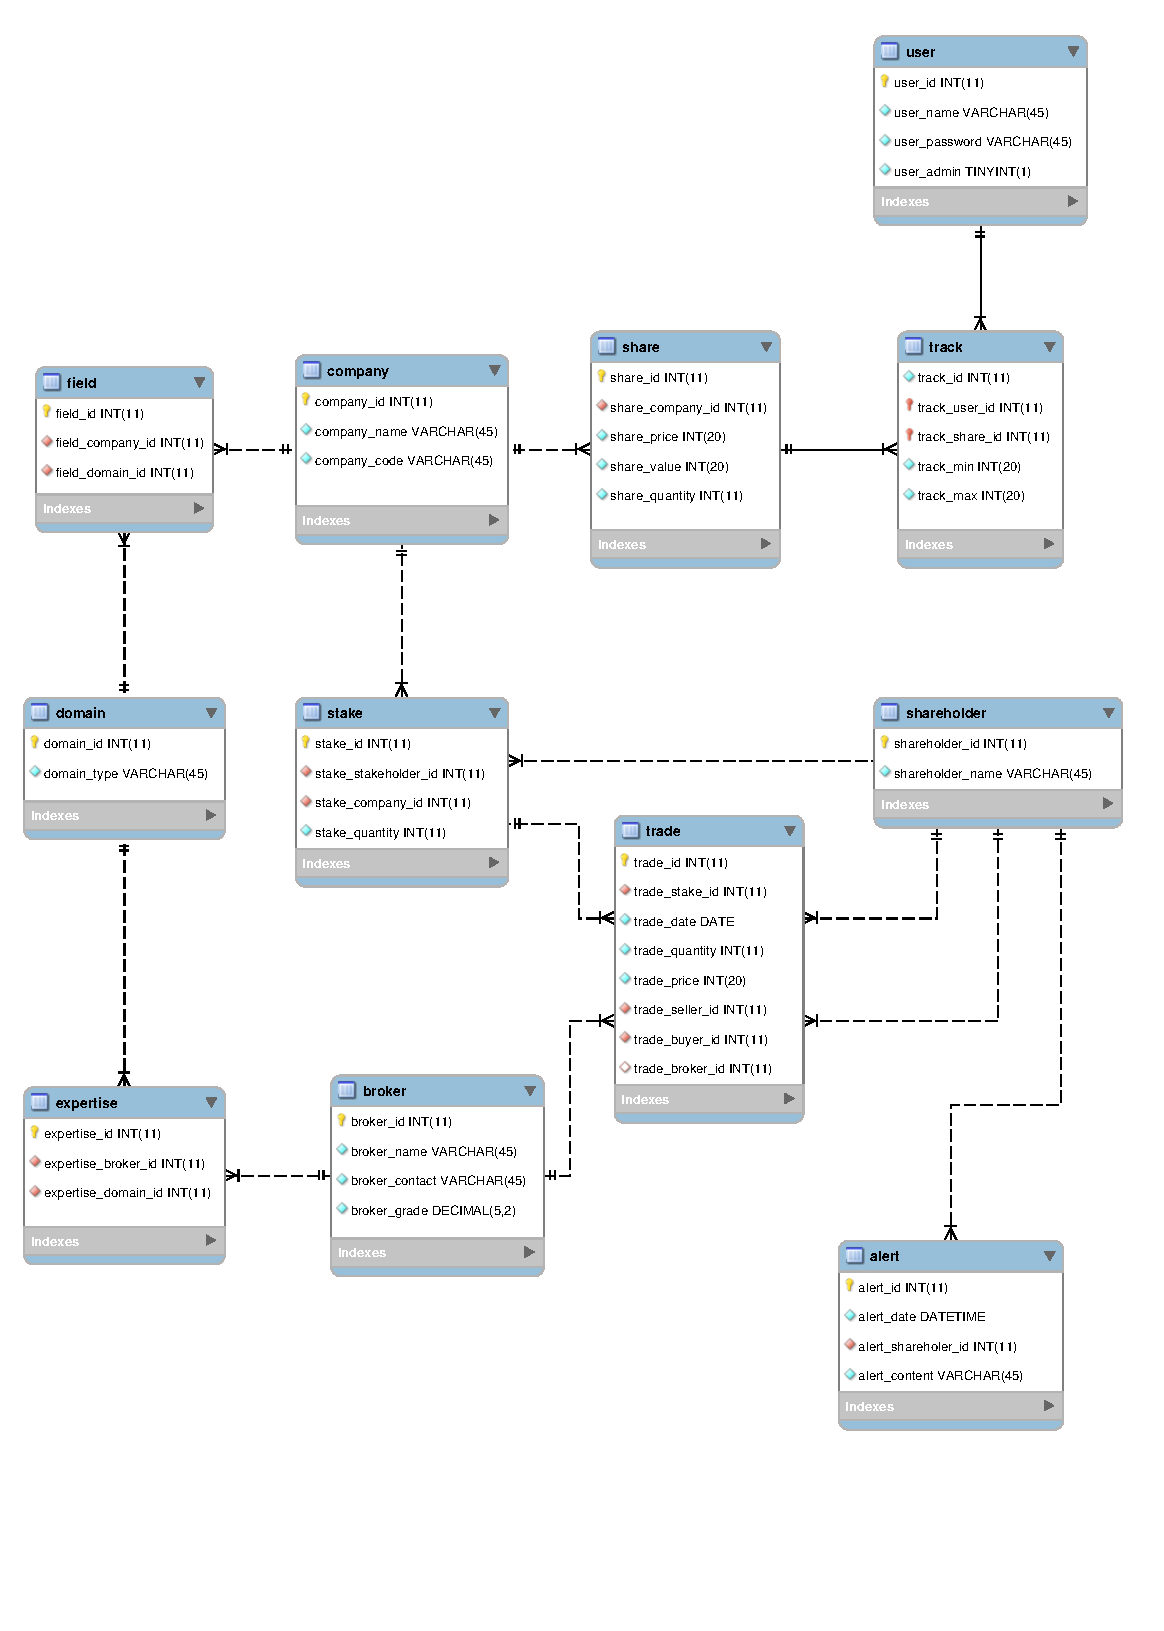
\includegraphics[width=\textwidth]{res/share_trader_er.pdf}
\label{ap-schema}


\section{Share Trader Use Case Diagram}
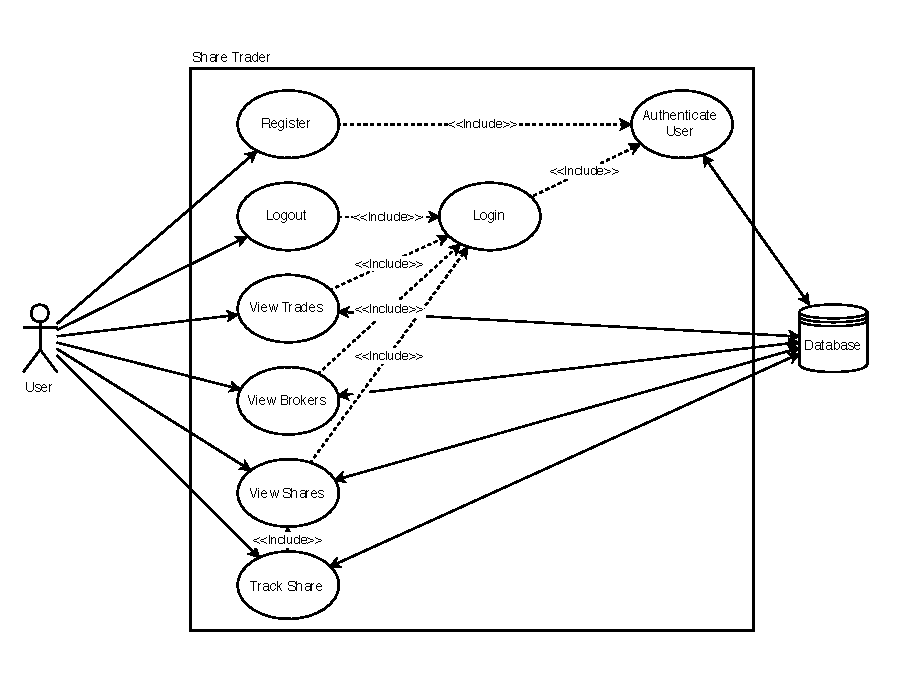
\includegraphics[width=\textwidth]{res/share_trader_uc.pdf}
\label{ap-uc}

\end{document}

